The dance of triangles on an elliptic arena is laden with bewilderement and suprise. 

This research started upon conversations with Jair Koiller about the geometry of elliptic billiard trajectories, following one author's recent work in control of heliostat fields for solar energy plants\footnote{Such fields are in fact a discretized/flattened focusing paraboloid, see \cite{sundrop2016,esolar2017}.}; see \cite{gross2020-solar} for a recent publication. An early, naïve experimental artifact was an animation of 3-periodics in the elliptic billiard along with the locus of their incenter; see  \cite{dsr_vid11incenter}. A natural choice given that each vertex is bisected by the ellipse normal. At the time we did not know this locus could be an ellipse, and indeed, how rare a find this is (we have conjecture that amongst the 5d space of possible ellipse pairs, only in the confocal pair -- a 1d subspace -- can the locus of the incenter be a conic). A twin animation was also produced depicting the self-intersected locus of the intouchpoints; see \cite{dsr_vid11e}.

Shortly thereafter \cite{olga14} produced a proof using methods of complex algebraic geometry.
%by complexification of the phenomenon. 
This was followed by an alternative    proof using techniques of real analytic   geometry given explicitly the equation of the locus; see \cite{garcia2019-incenter}. The loci centroids of Poncelet polygons was studied in \cite{schwartz2016-com}. In  \cite{garcia2019-incenter} the centroid locus was given explicitly.  Also \cite{corentin2021-circum} and \cite{garcia2018} proved that the locus of the circumcenter over billiard 3-periodics is also an ellipse.

\begin{figure}[H]
    \centering
    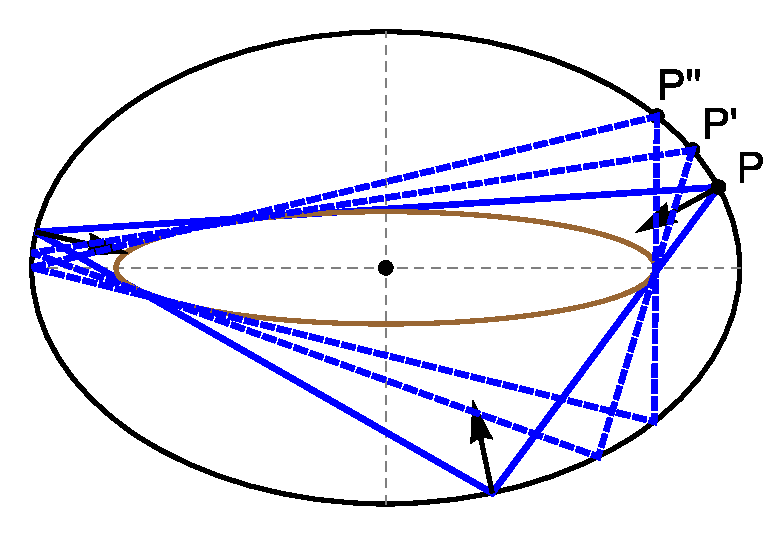
\includegraphics[width=.7\textwidth]{chap_01/pics/pics_01_030_three_orbits.eps}
    \caption{Billiard 3-periodics are a 1d family of Poncelet triangles interscribed between two confocal ellipses. By Graves' theorem, their internal angles are bisected by the outer ellipse's normals.}
    \label{fig:01-three-orbits-proof}
\end{figure}

\begin{figure}
    \centering
    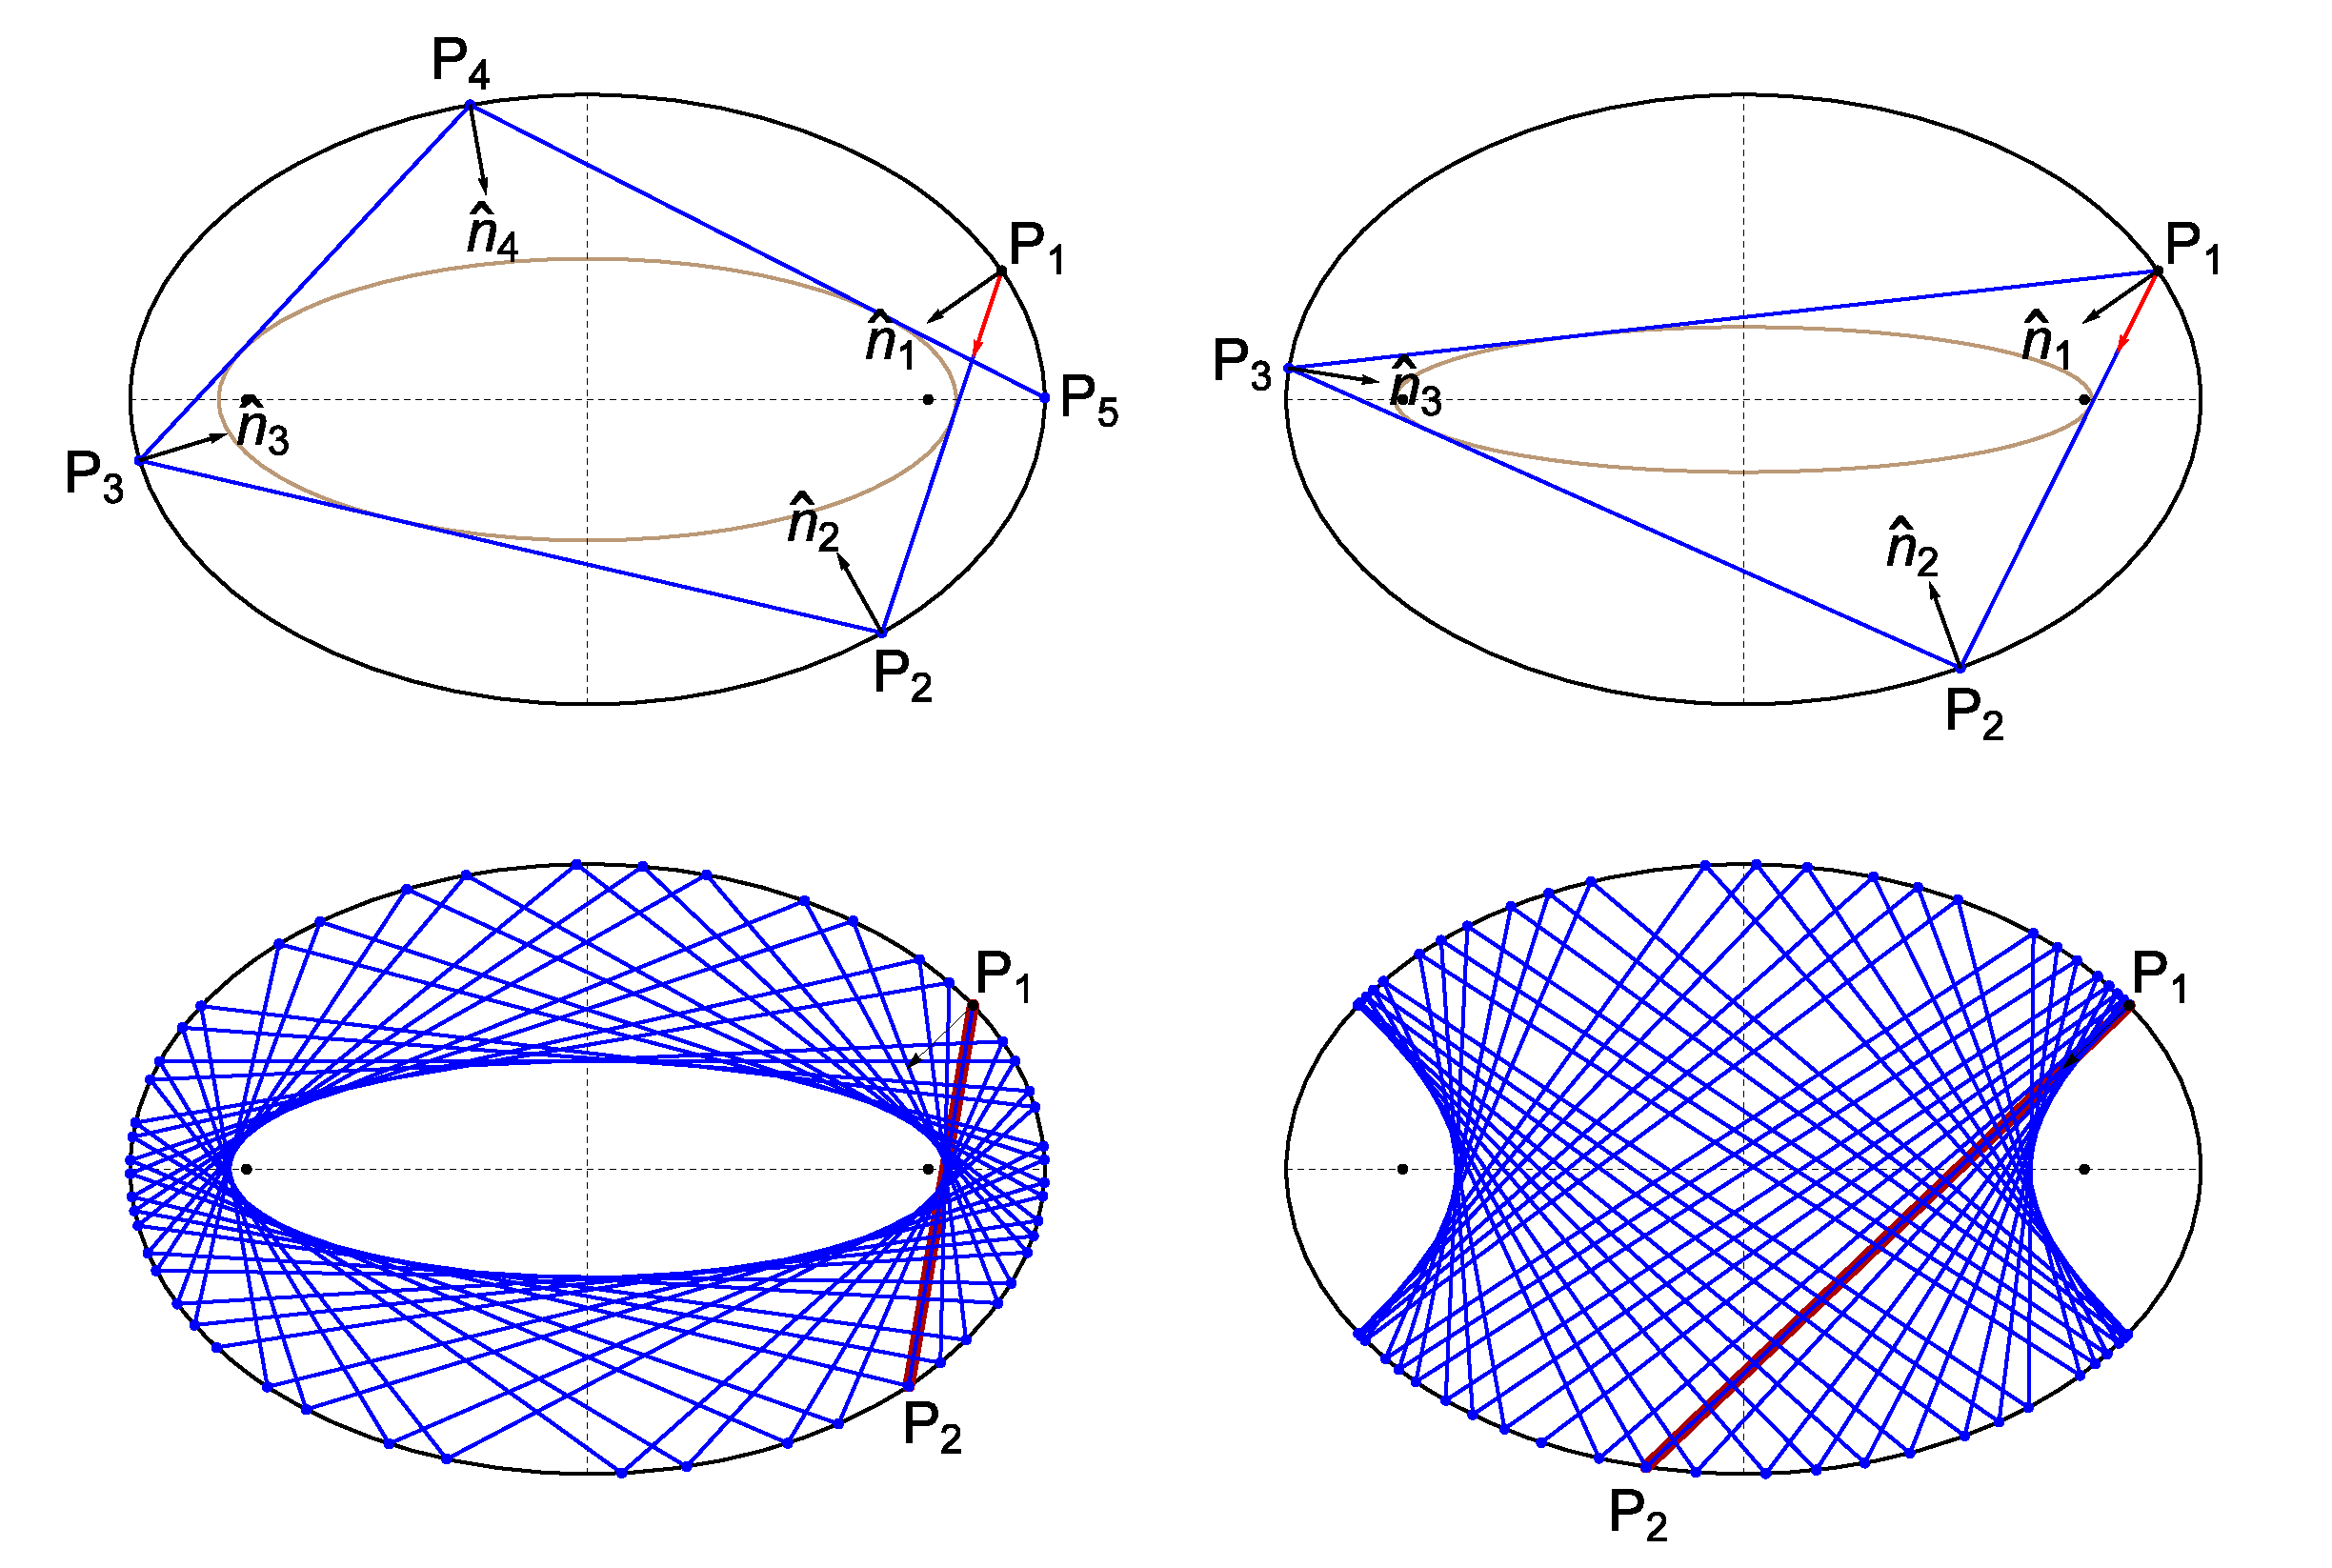
\includegraphics[width=\textwidth]{pics_01_010_billiard_trajectories.eps}
    \caption{Trajectory regimes in the elliptic billiard. \textbf{Top left}: The first four segments of a trajectory departing at $P_1$ and moving toward $P_2$, bouncing at $P_i, i=2,3,4$. At each bounce the normal $\hat{n}_i$ bisects incoming and outgoing segments. Joachimsthal's integral \cite{sergei91} means all segments are tangent to a confocal {\em caustic} (brown). \textbf{Top right}: All 3-periodic orbits are tangent to a confocal caustic (brown). \textbf{Bottom}: The first 50 segments of a non-periodic trajectory starting at $P_1$ and directed toward $P_2$. Segments are tangent to a confocal ellipse (left) or hyperbola (right). The former (respectively, latter) occurs if $P_1P_2$ passes outside (respectively, between) the elliptic billiard's foci (black dots). Early \href{https://youtu.be/A7mPzrNJHkA}{Video 1}, \href{https://youtu.be/9zAr5-nm7mw}{Video 2}, \href{https://youtu.be/6yXA0dyWhFY}{Video 3}}
    \label{fig:01-billiard-trajectories}
\end{figure}

%\begin{figure}
%    \centering
%    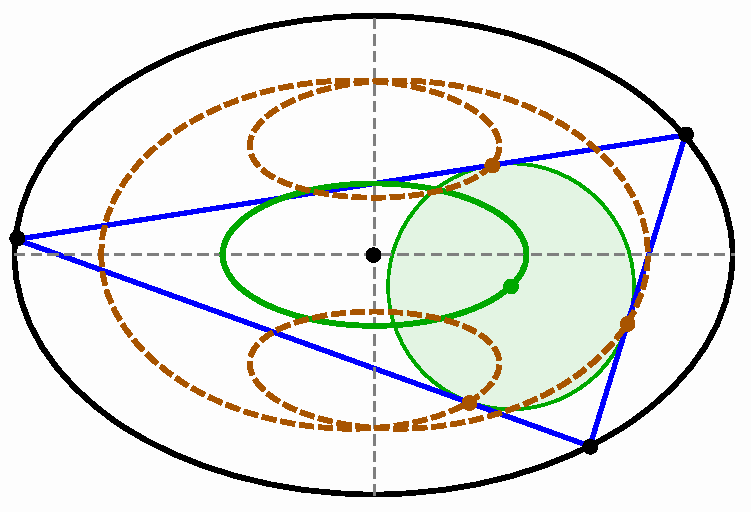
\includegraphics[width=.7\textwidth]{pics_01_020_intouch_locus.pdf}
%    \caption{A billiard 3-periodic (blue), its incircle (transparent green), incenter (green dot) and intouch points (brown dots). Over this 1d Poncelet family, the locus of the incenter locus is an ellipse (green), while that of the intouchpoints is a self-intersecting curve (dashed brown).
%    \href{https://youtu.be/9xU6T7hQMzs}{Video}}
%    \label{fig:01-intouch-locus}
%\end{figure}

\begin{figure}
    \centering
    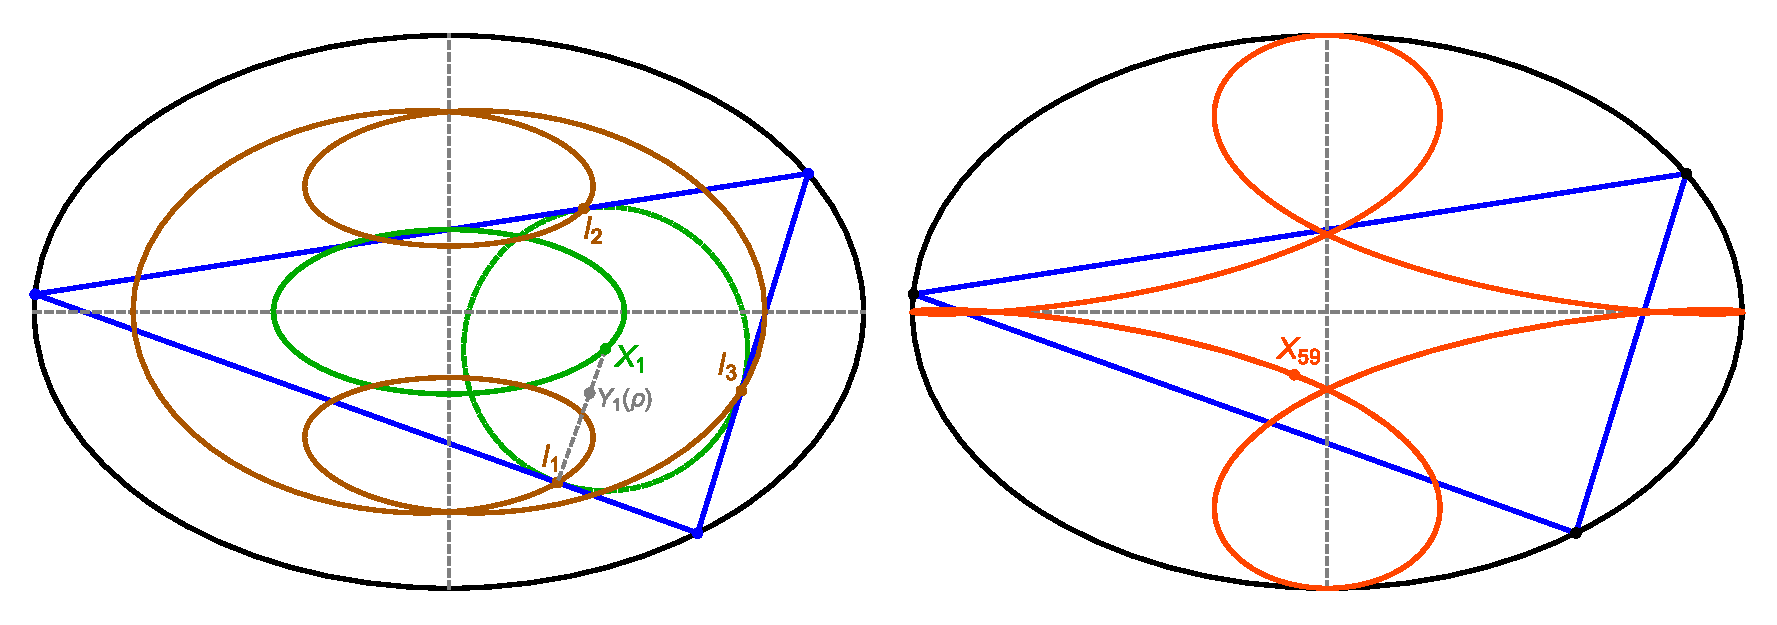
\includegraphics[width=\textwidth]{pics_01_040_x1_x59.eps}
    \caption{\textbf{Left}: Over billiard 3-periodics (blue), the locus of the incenter $X_1$ is an ellipse (green). However, that of the intouchpoints $I_1,I_2,I_3$, i.e., the points of contact of the incircle (dashed green) with the sidelines, is a self-intersecting curve (brown). \href{https://bit.ly/3q4b0Nn}{app},  \href{https://youtu.be/BBsyM7RnswA}{Video 1}, \href{https://youtu.be/9xU6T7hQMzs}{Video 2}. \textbf{Right}: The locus of $X_{59}$, i.e., the Isogonal conjugate of the Feuerbach point, is a curve (orange) with four self-intersections.
    \href{https://bit.ly/3i4h6dX}{app}}
    \label{fig:01-intouch-x59}
\end{figure}
 
 
